\documentclass[11pt]{article}
\usepackage{amsthm, bookmark, pgfplots, amsmath,textcomp,amssymb,geometry,graphicx,enumerate, mathtools, braket, hyperref, float, listings}
\usepackage[makeroom]{cancel}

\def\Name{Brandon Finley}  % Your name
\def\Homework{7} % Number of Homework
\def\Session{Fall 2020 } % Semester and year
\def\CRS{APPM 5515: High Dimensional Probability}% Course number : course name
\renewcommand\qedsymbol{$\blacksquare$}

\title{\CRS -- \Session --- Homework \Homework} % Course number : course name -- \
\author{\Name}
\markboth{\CRS--\Session\  Homework \Homework\ \Name}{\CRS-- \Session\-- Homework \Homework\ -- \Name}
\pagestyle{myheadings}
\date{}

\textheight=9in
\textwidth=6.5in
\topmargin=-.75in
\oddsidemargin=0.25in
\evensidemargin=0.25in
\setlength\parindent{0pt}
\allowdisplaybreaks

\begin{document}
\maketitle

\begin{enumerate}
	\item Compute a bound for the second eigenvalue. \\
	if $v = n(p-q) > \sqrt{2n(p+q)}$, then $\lambda_2$ is no longer in the ``semi-circle.''
	And we know $\lambda_2 = \frac{n(p-q)}{2} + \frac{p + q}{p - q}$. So the question boils down to the following
	\begin{equation}
		\text{is } \lambda_2 = \frac{n(p-q)}{2} + \frac{p + q}{p - q} > \sqrt{2n(p+q)} \text{ ?}
	\end{equation}
	We can extend this to say
	\begin{align*}
		\frac{n(p-q)}{2} + \frac{p + q}{p - q} &> \frac{\sqrt{2n(p+q)}}{2} + \frac{p + q}{p - q} \\
		\implies \frac{p+q}{p-q} &\ge \frac{\sqrt{2n(p+q)}}{2} \\
		&= \sqrt{\frac{n(p+q)}{2}}
	\end{align*}
	which we can verify is true experimentally.
	\item
	If $p = \alpha \frac{\log n}{n}$ and $q = \beta \frac{\log n}{n}$.
	\begin{align*}
		\implies n \left( \alpha \frac{\log n}{n} - \beta \frac{\log n}{n} \right) &> \sqrt{2n \left( \alpha \frac{\log n}{n} + \beta \frac{\log n}{n} \right) } \\
		\implies \log(n)(\alpha - \beta) &> \sqrt{2 \log (n) \left( \alpha + \beta \right)}\\
		\implies \alpha - \beta &> \frac{\sqrt{2(\alpha + \beta)}}{\sqrt{\log(n)}} = \frac{2}{\sqrt{\log(n)}} \sqrt{\frac{\alpha + \beta}{2}}
	\end{align*}
	\item In practice $p \ll \frac{\log(n)}{n}$ so it is better to write $p = a/n$ and $q=b/n$. Thus we can say the following
	\begin{align*}
		\implies n \left( \frac{a}{n} - \frac{b}{n}\right) &> \sqrt{2n \left( \frac{a}{n} + \frac{b}{n} \right)} \\
		\implies a - b &> \sqrt{2(a + b)} \\
		\implies \frac{a - b}{2} &> \frac{\sqrt{2(a + b)}}{2} = \sqrt{\frac{a + b}{2}}
	\end{align*}
	\item If $w^{~} = w$, then $\delta_{w_i^{~}, w_i} = 1$ and $\delta_{-w_i^{~}, w_i} = 0$. Thus,
	\begin{align*}
		\text{rawoverlap} &= \max \left( \sum_{i=1}^n \delta_{w_i^{~}, w_i}, \sum_{i=1}^n \delta_{-w_i^{~}, w_i}\right) \\
		&= \max \left( \sum_{i=1}^n 1, 0\right) \\
		&= \max (n, 0) = n \\
		&\implies \text{overlap} = \frac{2}{n} \cdot \text{rawoverlap} - 1 = \frac{2n}{n} - 1 = 1
	\end{align*}
	We also note that if we randomly partition our nodes, that is, we have that $w_i = {-1, 1}$ with $p_i = 0.5$, we can show that then the expected value of
	$\delta_{w_i^{~}, w_i} = \delta_{-w_i^{~}, w_i} = \frac{1}{2}$ and so we have that
	\begin{align*}
		\text{rawoverlap} &= \max \left( \sum_{i=1}^n \delta_{w_i^{~}, w_i}, \sum_{i=1}^n \delta_{-w_i^{~}, w_i}\right) \\
		&= \max \left( \sum_{i=1}^n \frac{1}{2}, \sum_{i=1}^n \frac{1}{2} \right) \\
		&= \max \left( \frac{n}{2}, \frac{n}{2}\right) \\
		&= \frac{n}{2} \\
		&\implies \text{overlap} = \frac{2}{n} \cdot \text{rawoverlap} - 1 = \frac{2}{n} \cdot \frac{n}{2} - 1 = 0
	\end{align*}
	\item Now, onto the code we have written to validate our findings in this and the last Homework. \textit{Note: The axis correspond to the indices of the matrix, so when $\alpha = 0$ on the graph, $\alpha = 5$. Likewise, when $\beta = 0$ on the graph, $\beta = 1$}.
	Also note that the values I got for the network where it was near 0, was not completely zero. This was different from what was seen in the problem set. Thus, it caused the decision boundary curve to be slightly higher than what seems it should be. I wonder why the values were close to zero but not exactly zero, especially for the dense network. Anyways, we have the dense network:
	\begin{figure}[H]
	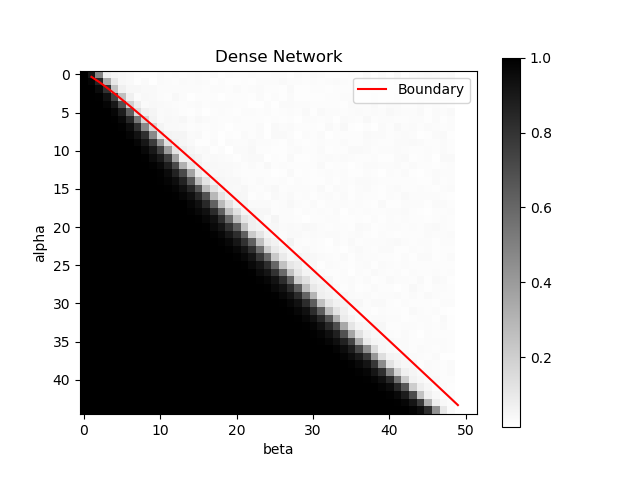
\includegraphics[width=12cm]{DenseScoreGraph.png}
	\centering
	\end{figure}
	Along with the sparse network:
	\begin{figure}[H]
	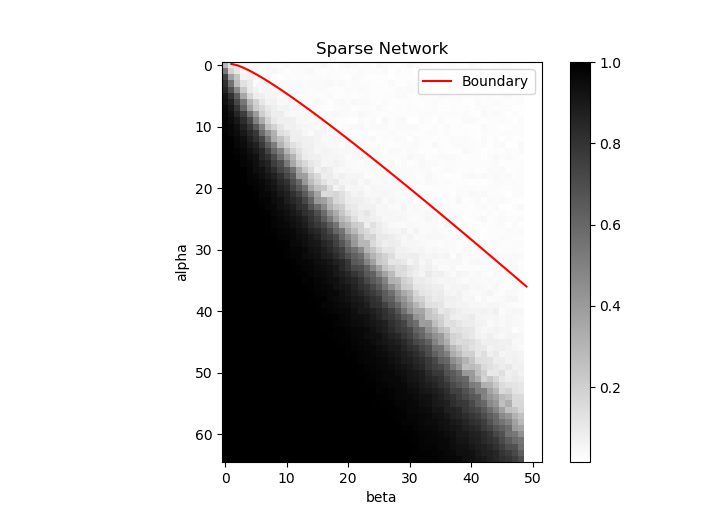
\includegraphics[width=12cm]{SparseScoreGraph.png}
	\centering
	\end{figure}
	And finally, using the same method on Zachary's karate club, we have that score $=1$ with the following prediction, where a community value of 1 corresponds to community 1 and -1 corresponds to community 2. Although, since we just care about the partitions, they have arbitrary meanings.
	\begin{center}
	\begin{tabular}{|c|c|}
	\hline
	Node & Community \\
	\hline
	1 & 1 \\
	2 & 1 \\
	3 & 1 \\
	4 & 1 \\
	5 & 1 \\
	6 & 1 \\
	7 & 1 \\
	8 & 1 \\
	9 & -1 \\
	10 & -1 \\
	11 & 1 \\
	12 & 1 \\
	13 & 1 \\
	14 & 1 \\
	15 & -1 \\
	16 & -1 \\
	17 & 1 \\
	18 & 1 \\
	19 & -1 \\
	20 & 1 \\
	21 & -1 \\
	22 & 1 \\
	23 & -1 \\
	24 & -1 \\
	25 & -1 \\
	26 & -1 \\
	27 & -1 \\
	28 & -1 \\
	29 & -1 \\
	30 & -1 \\
	31 & -1 \\
	32 & -1 \\
	33 & -1 \\
	34 & -1 \\
	\hline
	\end{tabular}
	\end{center}
\end{enumerate}
\begin{center}
	\boxed{{\textbf{| END |}}}
\end{center}
\end{document}

[ 1  1  1  1  1  1  1  1 -1 -1  1  1  1  1 -1 -1  1  1 -1  1 -1  1 -1 -1
 -1 -1 -1 -1 -1 -1 -1 -1 -1 -1]